% !TeX program = xelatex

% Chat GPT's universal template for Latin, Cyrillic, Arabic, and Hebrew environments using XeLaTeX.

\documentclass[12pt]{article}
% ===== Packages ===============================================
\usepackage{fontspec}     % For OpenType/Unicode fonts
\usepackage{polyglossia}  % For multilingual support
\usepackage{amsmath}
\usepackage{amsfonts}
\usepackage{amssymb}
\usepackage{graphicx}
\usepackage{float}
\usepackage{tabularx}
\usepackage{xspace}
\usepackage{tipa}
\usepackage{dirtree}
\usepackage{url}
\usepackage{color}
\usepackage[toc,page]{appendix}
\usepackage[colorlinks=false, pdfborder={0 0 0}]{hyperref}
\usepackage[left=2.30cm, right=1.50cm, top=2.00cm, bottom=1.80cm]{geometry}
 \usepackage{enumitem}
\usepackage{lipsum}
\usepackage[toc,page]{appendix}

% Table packages
\usepackage{longtable}       % multipage tables
\usepackage{tabularx}        % adjustable-width columns
\usepackage{ltablex}         % cross of longtable+tabularx
\keepXColumns

% ===== Multilingual environments ==============================
% -------------------------
% Languages
% -------------------------
\setmainlanguage{english}					% Main language
\setotherlanguages{hebrew,arabic,russian}	% Other languages

% -------------------------
% Fonts
% -------------------------
% \setmainfont{Latin Modern Roman}							% Latin script serif
\setmainfont{ClearSans}               						% Latin script sans
\newfontfamily\cyrillicfont{Times New Roman}   				% Cyrillic
\newfontfamily\hebrewfont[Script=Hebrew]{Alef}      		% Hebrew
\newfontfamily\arabicfont[Script=Arabic]{Noto Naskh Arabic} % Arabic

% --------------------------------------
% Custom environments for RTL paragraphs
% --------------------------------------
% Hebrew paragraph
\newenvironment{HebrewParagraph}
{\begin{RTL}\hebrewfont}
	{\end{RTL}}

% Arabic paragraph
\newenvironment{ArabicParagraph}
{\begin{RTL}\arabicfont}
	{\end{RTL}}

% Cyrillic paragraph (optional)
\newenvironment{CyrillicParagraph}
{\cyrillicfont}
{}

% ===== Inline Multilingual Text ===============================
%	\texthebrew{שלום עולם}			% Hebrew inline
%	\textarabic{مرحبا بالعالم}		% Arabic inline
%	\textrussian{Привіт, світе!}	% Cyrillic inline

% ===== Multilingual Paragraphs ================================
%\begin{HebrewParagraph}
%זהו פסקה מלאה בעברית.
%ניתן להקליד כאן יותר משורה אחת.
%\end{HebrewParagraph}
%
%\begin{ArabicParagraph}
%هذا فقرة كاملة بالعربية.
%يمكن كتابة أكثر من سطر هنا.
%\end{ArabicParagraph}
%
%\begin{CyrillicParagraph}
%	Це повний абзац українською.
%	Можна писати більше одного рядка.
%\end{CyrillicParagraph}

% ===== Multilingual Mixed Text ================================
% Here is mixed text: \texthebrew{שלום}, \textarabic{مرحبا}, and English together.

% USAGE DIRTREE
%==============
%\dirtree{%
	%	.1 Root.
	%	.2 Level 2 \DTcomment{Level 2 comment}.
	%	.3 Level 3 \DTcomment{Level 3 comment}.
	%}

% USAGE TABULARX
%================
%\begin{tabularx}{0.95\textwidth}{|l|X|}
%	\hline
%	Header 1	& Header 2		\\
%	\hline
%	Line 1 Left	& Line 1 Right 	\\
%	Line 2 Left	& Line 2 Right 	\\
%	\hline
%\end{tabularx}

%USAGE ITEMIZE WITH ITEMSEP
%==========================
%\begin{itemize}\itemsep-4pt
%\item First Item
%\item Second Item
%\item ...
%\item Last Item
%\end{itemize}

% USAGE APPENDICES
%=================
%\appendices
%\section{Important Equations}

% MATRICES
%=========
% matrix		no borders
% pmatrix		()
% bmatrix		[]
% vmatrix		||
% Vmatrix		|| ||
% BMatrix		{}

% ALIGNMENT
% =========
% \begin{equation}\label{key}
	% 	\begin{aligned}
		% 		a   &= x_{ij} \\
		% 		b_j &= y_j 
		% 	\end{aligned}
	% \end{equation}

% AUTO COUNTER (the prefix here being "Requirement")
%===================================================
\newcounter{ReqCounter}
\newcommand{\req}{\protect\stepcounter{ReqCounter}\textbf{RQ} \textbf{\theReqCounter.}~}

%============= Macros ===============
\newcommand{\gw}{groundwater\xspace}
\newcommand{\Gw}{Groundwater\xspace}
\newcommand{\dd}{drawdown\xspace}
\newcommand{\Dd}{Drawdown\xspace}
\newcommand{\gf}{geofiltration\xspace}
\newcommand{\Gf}{Geofiltration\xspace}
\newcommand{\cd}{conductifity\xspace}
\newcommand{\Cd}{Conductifity\xspace}
\newcommand{\pz}{piezoconductifity\xspace}
\newcommand{\Pz}{Piezoconductifity\xspace}

\newcommand{\rc}{recharge\xspace}
\newcommand{\ip}{impermeable\xspace}
\newcommand{\bd}{boundary\xspace}
\newcommand{\fl}{flow\xspace}

\newcommand{\ds}{dynamical system\xspace}
\newcommand{\dss}{dynamical systems\xspace}
\newcommand{\Dss}{Dynamical systems\xspace}
\newcommand{\lds}{linear dynamical system\xspace}
\newcommand{\ldss}{linear dynamical systems\xspace}

\newcommand{\lt}{Laplace transform\xspace}
\newcommand{\lti}{Laplace transform inversion\xspace}
\newcommand{\lop}[1]{\mathcal{L}\{#1\}\xspace}			% Laplace transform operator		
\newcommand{\ilop}[1]{\mathcal{L}^{-1}\{#1\}\xspace}	% Inverted Laplace transform operator

\newcommand{\ode}{ordinary differential equation\xspace}
\newcommand{\odes}{ordinary differential equations\xspace}
\newcommand{\pde}{partial differential equation\xspace}
\newcommand{\pdes}{partial differential equations\xspace}

\newcommand{\tmp}{temporal\xspace}
\newcommand{\tf}{transfer function\xspace}
\newcommand{\tfs}{transfer functions\xspace}
\newcommand{\Tf}{Transfer function\xspace}


% -------------------------
% Document
% -------------------------
\author{Stanislav Koncebovski}
\title{Laplace Transform}

\begin{document}
	\maketitle
	
	\section{Definitions}
	% \lop{g(t)} \\ \ilop{H(p)}
	One of very useful tools for the description of the behavior of \ldss is the \lt. Here we render a few general definition of this instrument and point to those of its properties that find application for those purposes. We limit ourselves to a mere enumeration of the facts, with a minimum of evaluation or proof. Readers interested in strict mathematical results are referred to a host of available literature (e.g. \cite{davies_integral_2002}).
	
	\lt is defined for functions of time $f(t)$ with the following properties:
	\begin{itemize}\itemsep-4pt
	\item $f(t) = 0, t < 0;$
	\item for $t \rightarrow \inf$, $f(t)$ either decreases or, if it increases, then no faster than some exponential, $f(t) \leq e^{\alpha t}, \alpha > 0.$
	\end{itemize}
	Functions of time occurring in \ldss normally fulfill both of these conditions.
	
	If these conditions are fulfilled, the Laplace image of $f(t)$ is defined as
	
	\begin{equation}\label{eq:lablace basic}
		F(p) = \int \limits_0^\infty e^{-pt} f(t) dt.
	\end{equation}
	
	The function $F(t)$ is then called the Laplace original of $F(p).$
	
	Often the fact that $F(p)$ is the Laplace image of $f(t)$ is represented in operator notation:
	\begin{equation}
		F(p) = \lop{f(t)}.
	\end{equation}
	
	The other way round, if we want to state that $f(t)$ is the Laplace original of $F(p)$ we can express it with the following operator notation:
	\begin{equation}
		f(t) = \ilop{F(p)}.
	\end{equation}
	
	\section{Some properties of \lt}
	\paragraph{Linearity\\}
	\lt is linear, that is the principle of superposition fulfills (obviously, due to the linearity of the operation of integration):
	\begin{equation}\label{eq:laplace lineariry}
	 	\begin{aligned}
	 		\lop{f_1(t) + f_2(t)}  &= \lop{f_1(t)} + \lop{f_2(t)}, \\
	 		\lop{k \cdot f(t)} &= k \cdot \lop{f(t)}, k = const.
	 	\end{aligned}
	\end{equation}
	
	\paragraph{\lt of derivative\\}
	If the \lt for a function is known, \lt for its derivative can be found in a simple expression. Indeed,
	\[ 
		\lop{f'(t)} = \int \limits_0^\infty e^{-pt} f'(t) dt.
	\] 
	Applying the rule of partial integration ($e^{-pt} = u, ~ f't) dt = dv$), we obtain that 
	\[ \lop{f'(t)} = e^{-pt} f(t) \rvert_0^\infty + p \int \limits_0^\infty e^{-pt} f(t) dt, \] in other words,
	
	\begin{equation}
		\lop{f'(t)} = p \lop{f(t)} - f(0).
	\end{equation}
	
	If, additionally, $f(0) = 0$ (which is very often if the model is interested in deviations from some initial value - \gw \dd being an example), we have
	\begin{equation}\label{eq: laplace of derivative}
		\lop{f'(t)} = p \cdot \lop{f(t)}.
	\end{equation}
	
	\paragraph{\lt of higher derivatives\\}
	Analog to how the expression for the \lt of the first derivative was obtained, the same technique can be applied to obtain expressions for the \lt of higher derivatives. For example,
	\begin{equation}\label{eq: lt of higher derivatives}
		\begin{aligned}
			\lop{f''(t)} &= p^2 \lop{f(t)} - f'(0) p - f(0), \\
			\lop{f'''(t)} &= p^3 \lop{f(t)} - f''(0) p^2 - f'(0) p - f(0), \\
			etc.&~
		\end{aligned}
	\end{equation}
	
	\paragraph{\lt of integral\\}
	Let $g(t) = \int \limits_0^t f(\tau) d \tau$ be the integral function of $f(t.)$ The \lt of $g(t)$ can then be expressed in terms of $\lop{f(t)}.$ Indeed, applying the rule of partial integration to the expression
	
	\[
		\int \limits_0^\infty e^{-pt} g(t) dt
 	\]
 	
 	we let $e^{-pt} dt = dv,~ g(t) = u.$ Then $v = -\frac{1}{p} \cdot e^{-pt}, ~ du = \frac{dg}{dt} \cdot dt = f(t) dt,$ and
 	
 	\[ 
 		\lop{g(t)} = -\frac{1}{p} \cdot g(t) \cdot e^{-pt} \rvert_0^\infty + \frac{1}{p} \cdot \int \limits_0^\infty e^{-pt} f(t) dt,
 	\]
 	
 	or
 	
 	\begin{equation}\label{eq: lt of integral}
 		\lop{\int \limits_0^t f(\tau) d \tau} = \frac{1}{p} \cdot \lop{f(t)}.
 	\end{equation}
 	
 	\paragraph{\lt of repeated integral\\}
 	Analog to how the expression for the \lt of the integral of a function was obtained, the same technique can be applied to obtain expressions for the \lt of repeated integrals. For example, if $g(t) = \int \limits_0^t f(\tau) d \tau,$
 	
 	\begin{equation} 
 		\lop{\int \limits_0^t g(\sigma) d \sigma} = \frac{1}{p^2} \cdot \lop{f(t).}
 	\end{equation}
 	
 	\paragraph{Limit values\\}
 	The values ​​of the original $f(t)$ at $t = 0$ and $t \rightarrow \inf$ an be determined using the image $F(p) = \lop{f(t)}$ as follows:
	\begin{equation}
		\begin{aligned}
			f(0) &= \lim_{p \to \infty} p F(p), \\
			f(\infty) &= \lim_{p \to 0} p F(p). \\
		\end{aligned}
	\end{equation}
	
	\paragraph{Time shift\\}
	If $F(p = \lop{f(t)}),$ then the \lt of the same function shifted by the value $a$
 	along the time axis, $f(t - a), $ is given by the following expression:
 	\begin{equation}\label{eq: laplace shift}
 		\lop{f(t+a)} = e^{-pa} \cdot \lop{f(t).}
 	\end{equation}
 	To obtain this, it is sufficient to perform a simple substitution of variables in  equation [\ref{eq:lablace basic}]. (Notice at that the values of the shifted function are zero if $t \in [0, a]$!)
 	
 	
 	\section{Images of some basic functions}
 	\subsection{Heaviside's unitary step}
 	Heaviside's unitary step function is defined as 
 	
 	\begin{equation} \label{eq:heaviside}
 		H(t) = \left\{\begin{array}{ll} 		% 'll' aligns two columns to the left
 			0, & \text{if } t < 0. \\ 			% Use \text{} for text, & to separate
 			1, & \text{if } t \ge 0.
 			\end{array}
			\right.
 	\end{equation}
 	
 	Its \lt is 
 	\begin{equation}\label{eq:laplace heaviside}
 		\lop{H(t)} = \frac{1}{p}.
 	\end{equation}
 	
 	\subsection{Linear function}
 	For the linear function
 	\[
 		f(t) = \left\{\begin{array}{ll}
 			0, & \text{if } t < 0. \\
 			\alpha t, & \text{if } t \ge 0 ~(\alpha = const)
 		\end{array}
 		\right.
 	\]
 	the \lt is 
 	\begin{equation}\label{eq: lt linear}
 		\lop{\alpha t} = \frac{\alpha}{p}.
 	\end{equation}
 	
 	\subsection{Exponential function}
 	For the exponential function $f(t) = e^{\alpha t}$ the \lt is
 	\begin{equation}\label{eq: lt exponent}
 		\lop{e^{\alpha t}} = \frac{1}{p - \alpha}.
 	\end{equation}
 	
 	\subsection{Dirac's delta function}
 	Dirac's delta function is a so called generalized function that can only be defined as a limit of a series of "normal" functions. Because of the special importance of this function in many applications (it describes, among other properties, locations of infinitely small sources and sinks), it seems to be appropriate to explain it to some more extent.
 	
 	\begin{figure}[H]
 		\centering
 		\includegraphics[width=0.5\linewidth]{../figures/part_1/diracs_delta}
 		\caption{To the definition of Diracs delta function}
 		\label{fig:diracs-delta}
 	\end{figure}
 	
 	There are many possibilities to define Dirac's delta function. The simplest of them is to consider the sequence of step functions like those shown in Figure  \ref{fig:diracs-delta}:
 	
 	\begin{equation}
 		h_\varepsilon(t) = \left\{\begin{array}{ll}
 			\frac{1}{\varepsilon}, \text{if } 0 \leq t <= \varepsilon, \\
 			0 \mathrm{otherwise}
 		\end{array}
 		\right.
 	\end{equation}
 	
 	With any finite value of $\varepsilon$ the integral $\int \limits_0^\infty h_\varepsilon(t) dt, $ or the area below the $h_\varepsilon$ line preserves the value of 1.
 	
 	Dirac's delta function $ \delta(t)$ is regarded as the generalized limit of this sequence of $h_\varepsilon(t)$ with $t \rightarrow 0.$
 	
 	According to the equations [\ref{eq:laplace heaviside}], [\ref{eq:laplace lineariry}], [\ref{eq: laplace shift}] the \lt of $h_\varepsilon(t)$ at any finite value of $\varepsilon$ is
 	\[ 
 		\lop{h_\varepsilon(t)} = \frac{1-e^{-p\varepsilon}}{p\varepsilon}.
 	\]
 	
 	With $\varepsilon \rightarrow 0 $ the numerator of the latter equation approaches $p\cdot \varepsilon + o(p \varepsilon),$ therefore $\lim_{\varepsilon \to 0} \lop{h_\varepsilon(t)} = 1,$ in other words,
 	\begin{equation} \label{eq:lt delta}
 		\lop{\delta(t)} = 1.
 	\end{equation}
 	
 	\section{\lt and \odes}
 	\paragraph{Introductory example\\}
 	A number of simple models from different domains of science and technology are described by a first-order \ode with constant coefficient. Classical examples are charging/discharging of a capacitor through a resistor with an applied external voltage; population dynamics under external influx; Brownian motion; chemical kinetics; inertial elements in control systems; discharge of springs and many others.
 	
 	\begin{figure}[H]
 		\centering
 		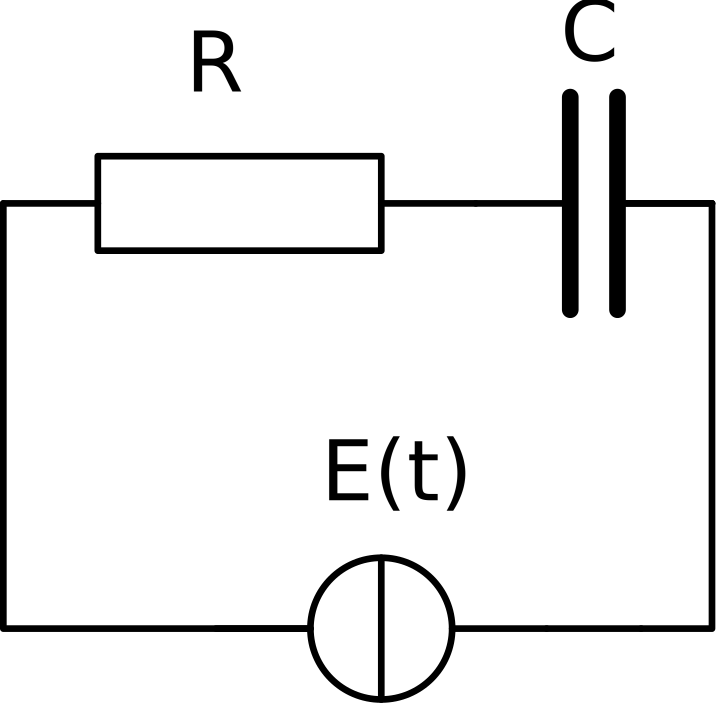
\includegraphics[width=0.25\linewidth]{../figures/part_1/RC-circuit}
 		\caption{Simple electrical circuit with a capacitor, resistor, and an external voltage source}
 		\label{fig:rc-circuit}
 	\end{figure}
 	
 	Figure \ref{fig:rc-circuit} shows a simple electrical circuit with a capacitor (C), resistor (R) and an external voltage source with a temporal dependency of the voltage value $E(t).$
 	
 	The temporal dependency of the voltage at the capacitor $V(t)$ is described by the following \ode \cite{Johnson_2014}:
 	\begin{equation}\label{eq:ode rc circuit}
 		\frac{dV}{dt} + \frac{1}{RC} V = \frac{1}{RC} \cdot E(t)
 	\end{equation}
 	
 	Let $\hat{V}(p)$ be the \lt of the temporal function $V(t)$: $\hat{V}(p) = \lop{V(t)}.$ According to [\ref{eq: laplace of derivative}] $\lop{\frac{dV}{dt}} = p \hat{V}(p) - V_0,$ where $V_0$ is the value of the capacitor voltage at the initial moment of time $t=0.$ The time dependency of the applied external voltage $E(t)$ is supposed to be known, as well as its \lt $\hat E(p).$ Applying \lt to both parts of [\ref{eq:ode rc circuit}], we obtain:
 	
 	\begin{equation}\label{eq:rc circuit lt}
 		p \hat{V}(p) - V_0 = \frac{1}{RC} \hat{V}(p) = \frac{1}{RC} \hat E(p).
 	\end{equation}
 	
 	Regrouping in [\ref{eq:rc circuit lt}] and setting $T = RC,$ we obtain the solution in terms of \lt:
 	\begin{equation}\label{eq:rc circuit solution in lt}
 		\hat{V}(p) = \frac{\hat E(p) + T V_0}{1 + Tp}.
 	\end{equation}
 	
 	Equation [\ref{eq:rc circuit solution in lt}] represents tie general solution of the \ode \ref{eq:ode rc circuit} in terms of \lt. Instead of a differential equation we have an algebraic equation now, and, if we are in a position to step down from a Laplace image to its temporal original, we can find the solution of the \ode for all cases. Finding  \tmp originals of arbitrary Laplace images will be considered in following sections; now let us dwell upon a few simple cases.
 	
 	\paragraph{Discharge of the capacitor with no external voltage\\}
 	In Equation [\ref{eq:rc circuit solution in lt}] let us set $\hat E(p) = 0$ (no external voltage.) Then
 	\begin{equation}
 		\hat{V}(p) = T V_0 \cdot \frac{1}{1 + Tp} = V_0 \cdot \frac{1}{1 + \frac{1}{T}}.
 	\end{equation}
 	
 	Comparing the right fraction of this expression with [\ref{eq: lt exponent}] we can easily conclude that the \tmp function of the capacitor voltage in this case is:
 	\begin{equation}\label{eq:rc-steady discharge example}
 		V(t) = V_0 \cdot e^{-t / T}.
 	\end{equation}
 	
 	Figure \ref*{fig:rcsteadydischarge} shows solution (\ref{eq:rc-steady discharge example}) computed using the \texttt{steady\_discharge} routine of the \texttt{RCCircuit} class (lilimod/electro/rc-circuit.py).
 	
 	\begin{figure}[H]
 		\centering
 		\includegraphics[width=0.75\linewidth]{../figures/part_1/rc_steady_discharge}
 		\caption{Capacitor discharge: time dependency of the capacitor voltage in the example ($V_0 = 100V, R=10000 \Omega, C = 10^{-4} F$)}
 		\label{fig:rcsteadydischarge}
 	\end{figure}
 	
 	\paragraph{Capacitor recharge\\}
 	Let us now consider the case when the capacitor is empty at $t=0$ ($V_0 = 0$) and the external voltage starts at $t=0$ and is constant furthermore: $E(t) = E_0 \cdot H(t)$.
 	
 	From (\ref{eq:rc circuit solution in lt}) we will have for this case:
 	\begin{equation}\label{eq:capacitor recharge lt}
 		\hat{V}(p) = \frac{E_0}{p} \cdot \frac{1}{1 + Tp} .
 	\end{equation}
 	We have already obtained that $\ilop{\frac{1}{1 + \frac{1}{T}}} = e^{-t/T}.$ The $\frac{1}{p}$ factor in (\ref{eq:capacitor recharge lt}) means that to obtain the Laplace original for $V(t)$ we first need to integrate this function (\ref{eq: lt of integral}):
 	\[ 
 		\ilop{\frac{1}{p} \cdot \frac{1}{1 + Tp}} = \int \limits_0^t e^{-\tau / T} d\tau = T (1 - e^{-t/T}),
 	\]
 	so that the time dependency of capacitor voltage will be
 	\begin{equation}
 		V(t) = E_0 \cdot (1 - e^{-t/T}).
 	\end{equation}
 	
 	\begin{figure}[H]
 		\centering
 		\includegraphics[width=0.75\linewidth]{../figures/part_1/rc_steady_recharge}
 		\caption{Capacitor recharge: time dependency of the capacitor voltage in the example ($V_0 = 100V, R=10000 \Omega, C = 10^{-4} F$)}
 		\label{fig:rcsteadyrecharge}
 	\end{figure}
 	
 	\paragraph{\lt for the solution of \odes: General case \\}
 	Analog to how we dealt in the above example, any \ode with constant coefficients can be transformed to an algebraic equation with respect to its \lt.
 	
 	Consider the linear \ode
 	\begin{equation}\label{eq: general linear ode}
 		a_{n} \frac{d^{n}X}{dt^{n}} + a_{n-1} \frac{d^{n-1}X}{dt^{n-1}} + ... + a_1 \frac{dX}{dt} + a_0 = E(t),
 	\end{equation}
 	where $a_n, ..., a_0 = \mathrm{const},$ $E(t)$ an arbitrary function of time. Due to (\ref{eq: lt of higher derivatives}), 
 	\[ 
 		\lop{\frac{d^{k}X}{dt^{k}}} = p^k \cdot \hat X(p) - \sum \limits_{i=0}^{k-1} p^i X^{(i)}_0,
 	\]
 	
 	where $\hat{X}(p) = \lop{X(t)},$ $X^{(i)}_0$ the initial values of the function $X(t)$ and its derivatives. Applying \lt to both parts of (\ref{eq: general linear ode}), we obtain:
 	\[
 		\left( \sum \limits_{k=0}^{n} a_k p^k \right) \cdot \hat X(p) = \hat E(p) + P_0(p),
 	\]
 	
 	where $\hat{E}(p) = \lop{E(t)}, $ $P_0(p)$ a polynomial of degree $n-1$ with coefficients being linear combinations of the initial values of the function $X(t)$ and its derivatives.
	
	In the special case when $P_0(p) = 0,$
	
	\begin{equation}
		\hat X(p) = U(p) \cdot \hat E(p),
	\end{equation}
	
	where
	\begin{equation}\label{eq: transfer function}
		U(p) = \frac{1}{\sum \limits_{k=0}^{n} a_k p^k}.
	\end{equation}
	
	In (\ref*{eq: transfer function}) $U(p)$ is called the transfer function \index{transfer function} of the \lds. For example, in (\ref{eq:capacitor recharge lt}) the \tf of the electrical system was
	\[ 
		U(p) = \frac{1}{1 + Tp},
	\]
	whereas the Laplace image of the constant external force was $\hat E(p) = E_0 / p.$
	
	\section{Inversion of \lt}
	Solution of \odes (and \pdes, as we will see later) is one of the main applications of \lt. Whereas it is relatively simple to get at a solution in terms of \lt, the next step is to convert them into temporal dependencies. This step is called \lti. We have already learned about a few elementary correspondences between \lt and \lti: (\ref{eq:laplace heaviside}) for the Heaviside function, (\ref{eq: lt linear}) for the linear function, (\ref{eq: lt exponent}) for the exponential function, and (\ref{eq:lt delta}) for Dirac's delta function. 
	
	Table (...) in Appendix contains more cases arises in concrete problems in \gf and similar contexts. There exist, besides, numerous collections of comprehensive inversion tables. Classical sources are, for example, \cite{Bateman_1954}, \cite{Abramowitz1964}, and many others..
	

	\section{Numerical Inversion of \lt}
		Despite the fact that the collection of \lt and its inversion is very ample, it is not always possible to find one in existing sources, especially by complicated or exotic \tmp dependencies of external forces. Fortunately, there also exists methods to find the numerical values of a Laplace original if the image is known. This class of methods is known as the numerical inversion of \lt.
		
		\subsection{Overview}
		A great number of methods for the numerical inversion of \lt has been developed in the last decades. The interested reader can find an overview of existing methods, among other publications, in \cite{davies_martin_1979}, \cite{cohen_numerical_2007}, \cite{kuhlman_2013}, \cite{piessens_1975}.
		
		According to the author's opinion, however, two methods stand out with respect of practical applications: the method of Harald Stehfest \cite{stehfest_1970} and the method of Peter den Iseger \cite{iseger_2006}. 
		%In the following sections we will dwell upon these two methods, and on one further historical method of Lev Gokhberg \cite{gokhberg_1982} included rather for private considerations.
		
		\subsection{Method of Stehfest}
		
		The method of Stehfest uses only the values of \lti om the real axis. This makes it a practical tool, since calculation of the image function with complex arguments causes sometimes greater difficulties. The method is based on an integration formula given by D.P. Gaver \cite{gaver_1966}:
	
		\begin{equation}\label{eq:stehfest}
			f(t) \approx \frac{\log 2}{t} \cdot \sum \limits_{i=1}^N V_i F\left( \frac{\log 2}{t} \cdot i \right),
		\end{equation}
		where
		
		\begin{description}[labelwidth=4em,leftmargin=!,itemsep=-4pt]
			\item[$f(t)$] the approximate value of the original at time value $t$,
			\item[$F(p)$] the Laplace image function,
			\item[$V_i$] the coefficients of integration in Gaver's equation,
			\item[$N$] the order of the integration formula.
		\end{description}
		
		The expression for the coefficients $V_i$ is as follows:
		\begin{equation}\label{eq: gaver coefficients}
			V_i = (-1)^{i + N/2} \cdot \sum \limits_{k = \left[ \frac{i + 1}{2} \right]}^{\min(i, N/2)} \frac{k^{N/2 + 1} (2k)!}{(N/2 - k)! k! (k-1)! (i-k)! (2k-i)!}
		\end{equation}
		
		Since the coefficients $V_i$ only depend on the value of $N$, so they only need to be calculated once. The value of $N$ must be even.
		
		The values of Stehfest's coefficients for a few values of $N$ are given in Table \ref*{tab:Stehfest coefficients}.
		
		\begin{table}[H]\label{tab:Stehfest coefficients}
			\centering
			\caption{Table of coefficients in Stehfest's inversion method fo a few values of $N$}
		\begin{tabular}{|r|r|r|r|r|r|r|}
			\hline
			i & N=2  & N=4     & N=6     & N=8            & N=10            & N=12\\
			\hline
			1 &  2.0 &   -2.0  &     1.0 &      -0.333333 &        0.083333 &  -1.666667e-02 \\
			2 & -2.0 &   26.0  &   -49.0 &      48.333333 &      -32.083333 &   1.601667e+01 \\
			3 &      &   -48.0 &   366.0 &    -906.000000 &     1279.000000 &  -1.247000e+03 \\
			4 &      &    24.0 &  -858.0 &    5464.666667 &   -15623.666667 &   2.755433e+04 \\
			5 &      &         &   810.0 &  -14376.666667 &    84244.166667 &  -2.632808e+05 \\
			6 &      &         &  -270.0 &   18730.000000 &  -236957.500000 &   1.324139e+06 \\
			7 &      &         &         &  -11946.666667 &   375911.666667 &  -3.891706e+06 \\
			8 &      &         &         &    2986.666667 &  -340071.666667 &   7.053286e+06 \\
			9 &      &         &         &                &   164062.500000 &  -8.005336e+06 \\
			10 &     &         &         &                &   -32812.500000 &   5.552830e+06 \\
			11 &     &         &         &                &                 &  -2.155507e+06 \\
			12 &     &         &         &                &                 &   3.592512e+05 \\
			\hline
		\end{tabular}			
		\end{table}
		

		
			A Python implementation of Stehfest's algorithm is contained in the \texttt{lilimod} library (\texttt{lilimaths/stehfest.py}).
			
			\subsubsection{Examples of application of Stehfest's method}
			
			\paragraph{Exponential Decay\\~}
			Laplace image: $F(p) = \frac{1}{1 + p}.$ Exact Laplace original: $f(t) = \E^{-t}.$ \\
			
			The results of numerical inversion are shown in Figure \ref{fig:stehfestexponentialdecay}. In this case, even with a relatively lower value of N=6 the results are already very accurate (maximum absolute deviation 0.0068 with $N=6$ at $t = 3.11.$)
			
			
			\begin{figure}[H]
				\centering
				\includegraphics[width=0.85\linewidth]{../figures/part_1/stehfest_exponential_decay}
				\caption{Results of numerical Laplace inversion by Stehfest's method for exponential decay.}
				\label{fig:stehfestexponentialdecay}
			\end{figure}
			
			\paragraph{Sine function\\}
			Laplace image: $F(p) = \frac{1}{1 + p^2}.$ Exact Laplace original: $f(t) = \sin t.$ \\
			
			The results of numerical inversion for this case shown in Figure \ref{fig:stehfestsine} behave differently as compared with the previous case. Whereas the deviation from the exact function in the beginning of the curve ($0 \leq t \lesssim 1.2 $) are reasonably accurate, accuracy drastically falls as the value of the argument grows. Even with the values of order as high as 22, the deviation from the exact solution becomes too high already after the first full oscillation (maximum absolute deviation 0.0339 with $N=22$ at $t = 5.01.$).		
			
			\begin{figure}[H]
				\centering
				\includegraphics[width=0.85\linewidth]{../figures/part_1/stehfest_sine}
				\caption{Results of numerical Laplace inversion by Stehfest's method for sine function.}
				\label{fig:stehfestsine}
			\end{figure}
			
			\paragraph{Damped sine function\\}
			Laplace image: $F(p) = \frac{1}{1 + (p+0.2)^2}.$ Exact Laplace original: $f(t) = \E^{-0.2 t}\sin t.$ \\
			
			\begin{figure}[H]
				\centering
				\includegraphics[width=0.85\linewidth]{../figures/part_1/stehfest_damped_sine}
				\caption{Results of numerical Laplace inversion by Stehfest's method for damped sine function.}
				\label{fig:stehfestdampedsine}
			\end{figure}
			
			The results of numerical inversion for the damped sine curve are shown in Figure \ref{fig:stehfestdampedsine}. Adding a little damping to the process improves the convergence, to an extent, as can bee seen from the behavior of the curves. Nevertheless, the deviations from the exact curve are still significant and tend to become greater as long as the value of time grows  (maximum absolute deviation 0.00311 with $N=22$ at $t = 4.71.$).		
			
			\paragraph{Linear growth\\}
			Laplace image: $F(p) = \frac{1}{p^2}.$ Exact Laplace original: $f(t) = t.$ \\
			
			\begin{figure}[H]
				\centering
				\includegraphics[width=0.85\linewidth]{../figures/part_1/stehfest_linear_growth}
				\caption{Results of numerical Laplace inversion by Stehfest's method for linear function.}
				\label{fig:stehfestlineargrowth}
			\end{figure}
			
			The results of numerical inversion are shown in Figure \ref{fig:stehfestlineargrowth}. For the case of linear function, even with a relatively lower value of N=6 the results are already very accurate (maximum absolute deviation 0.0107 with $N=6$ at $t = 5.01.$, $4.84 \cdot 10^{-6}$ with $N = 12$).		
			
			
			\paragraph{Asymmetric distribution\\}
			Laplace image: $F(p) = \frac{1}{(p + 1)^2}.$ Exact Laplace original: $f(t) = t \E^{-t}.$ \\
			\begin{figure}[H]
				\centering
				\includegraphics[width=0.85\linewidth]{../figures/part_1/stehfest_asymmetric_distribution}
				\caption{Results of numerical Laplace inversion by Stehfest's method for asymmetric distribution.}
				\label{fig:stehfestasymmetricdistribution}
			\end{figure}
			
			The results of numerical inversion are shown in Figure \ref{fig:stehfestasymmetricdistribution}. As can bee seen, the results become reasonably accurate with the values of $N \geq 10$ (maximum absolute deviation 0.00191 with $N=10$ at $t = 4.36.$).		
			
			
			\paragraph{Delayed unitary step\\}
			Laplace image: $F(p) = \frac{\E^{-p}}{p}.$ Exact Laplace original: $f(t) = H(t-1).$ \\
			
			\begin{figure}[H]
				\centering
				\includegraphics[width=0.85\linewidth]{../figures/part_1/stehfest_delayed_step}
				\caption{Results of numerical Laplace inversion by Stehfest's method for delayed unitary step.}
				\label{fig:stehfestdelayedstep}
			\end{figure}
			
			The results of numerical inversion are shown in Figure \ref{fig:stehfestdelayedstep}. Although the accuracy of the computed values of $f(t)$ with big values of time $t \geq 2.5 $can be considered as more or less accurate, behavior of the calculate curves in the vicinity of the original's breakpoint at $t = 1.$ This behavior cannot be improved by increasing of the order of integration. As can be seen from Table \ref{tab:Stehfest coefficients} the values if coefficients rapidly grow to very big values, as the order $N$ grows, which causes numerical instability due to rounding errors in the machine representation of float numbers.
			
			\paragraph{Rectangular wave\\}
			Laplace image: $F(p) = \frac{(\E^{-p} - \E^{-2p})}{p}.$ Exact Laplace original: $f(t) = H(t-1) - H(t-2).$ \\
			
			
			\begin{figure}[H]
				\centering
				\includegraphics[width=0.85\linewidth]{../figures/part_1/stehfest_rectanhular_wave}
				\caption{Results of numerical Laplace inversion by Stehfest's method for rectangular wave}
				\label{fig:stehfestrectanhularwave}
			\end{figure}
			
			Like in the case of delayed step, the behavior of the Stehfest approximated originals is far from satisfactory. Whereas in the vicinity of $t=0$ and with gig values of time the accuracy can be considered acceptable, the form of rectangular wave cannot be computed by Stehfest integration method. In this particular case, even the value of integration order as high as 26 did not do better. Further increase in the value of $N$ creates numerical instability, as is shown in Figure \ref{fig:stehfestrectanhularwaveunstable}.
			
			\begin{figure}[H]
				\centering
				\includegraphics[width=0.85\linewidth]{../figures/part_1/stehfest_rectanhular_wave_unstable}
				\caption{Numerical instability of Stehfest's method for rectangular wave with too high values of integration order.}
				\label{fig:stehfestrectanhularwaveunstable}
			\end{figure}
			
			Setting $N=28$ for the previous example created numerical instability illustrated by the chaotic cloud of black points in the right part of the graph in Figure \ref{fig:stehfestrectanhularwaveunstable}.
			
			\paragraph{Well function\\}
			Laplace image: $F(p) = \frac{1}{p} K_0\left( 2 \sqrt{0.8 p} \right).$ Exact Laplace original: $f(t) = 0.5 E_1\left( \frac{0.8}{t} \right).$ \\
			
			\begin{figure}[H]
				\centering
				\includegraphics[width=0.85\linewidth]{../figures/part_1/stehfest_well_function}
				\caption{Results of numerical Laplace inversion by Stehfest's method for the well function}
				\label{fig:stehfestwellfunction}
			\end{figure}
			
			The results of numerical inversion are shown in Figure \ref{fig:stehfestwellfunction}. As can bee seen, the results become quite accurate already with the values of $N \geq 6$ (maximum absolute deviation 0.0021 with $N=6$ at $t = 1.01.$).		
			
		\subsection{Method of den Iseger}
%		The method of den Iseger \cite{iseger_2006} realizes a version of Gaussian quadrature with complex values of the integrated function. It can also take into consideration singularities of the image function.
%		An array of the values of the image function computed in a number of defined nodes on the complex plane is then processed using inverted fast Fourier transform techniques and summed multiplied with defined weight factors.
		
%		The nodes of the quadrature formula and the summation weights are predefined for a number of typical cases and can be used directly.
		The method of den Iseger \cite{iseger_2006} realizes a version of Gaussian quadrature with complex values of the integrated function. Below is presented the algorithm of den Iseger's method according to \cite{tijms_2003}, for the mathematical intricacies the interested reader can look up the seminal paper \cite{iseger_2006} itself.
		
		The idea of den Iseger's method is the approximation of the original function $f(t)$ for the values of the time argument $t_k = k \Delta$, where $\Delta$ is the time step and $k = 0, ..., M-1,$ $M$ being the desired number of steps ($\Delta \cdot (M-1) = t_{fin},$) $t_{fin}$ the length of the time interval. The values $f(t_k)$ are approximated as 
		\begin{equation}\label{eq:tijms basic sum}
			f(t_k) \approx \frac{\E^{b k}}{\Delta} \sum \limits_{j=1}^n \alpha_j \int \limits_{-1}^1 \mathrm{Re} \left[ F(\frac{b + i \lambda_j + i \pi t}{\Delta}) \right] \cdot \cos \left( \pi k (t + 1) \right) dt,
		\end{equation}
		
		where $i = \sqrt{-1}.$ The values of $b$ and $n$ in (\ref{eq:tijms basic sum}) must be chosen appropriately (see below). The values $\lambda_j$ and $\alpha_j$ are the abscissae and the weights of the integration formula that only depend on n. To practically calculate using equation (\ref{eq:tijms basic sum}), the following algorithm is suggested:
		\paragraph{Input:} $F(p)$: Laplace image function; $\Delta$: time step; $M$: number of time points.
		\paragraph{Step 1} For $q = 0, ..., 2m$ and $j = 1, ..., n$ calculate
		\begin{equation}
			F_{jq} = \mathrm{Re} \left[ F \left( \frac{b + i \lambda_j + i \pi (q / m - 1)}{\Delta} \right) \right]
		\end{equation}
		and
		\begin{equation}
			F_q = \sum \limits_{j=1}^n \alpha_j F_{jq}, ~ q = 0, ... , 2m.
		\end{equation}
		
		\noindent Then let 
		\begin{equation}
			\hat g_k = F_k, ~ k = 1, ..., 2m - 1, ~ \hat g_0 = \frac{1}{2} (F_0 + F_{2m}).
		\end{equation}
		
		\paragraph{Step 2} Apply the inverse Fast Fourier Transform method to the vector $(\hat g_0, ..., \hat g_{2m-1})$. The result is the vector $(g_0, ..., g_{2m-1}).$
		
		\paragraph{Step 3} The resulting values of the original are
		\begin{equation}
			f(k \Delta) = \frac{2 \E^{b k}}{\Delta} \cdot g_k, k = 0, ..., M - 1.
		\end{equation}
		
		\paragraph{Selection of the values $b$ and $m$\\}
		To obtain best results, is is recommended \cite{tijms_2003} to select the value of $M$ as a power of 2. Then the value of $m$ is set to
		\begin{equation}
			m = 4 M
		\end{equation}
		and
		\begin{equation}
			b = \frac{22}{m}.
		\end{equation}
		The latter equation is derived as the result of numerical experiments \cite{tijms_2003}.
		
		As will be illustrated in the examples below, the accuracy of den Iseger's method is overwhelming, even for 'bad behaved' functions. As is indicated in \cite{tijms_2003}, for smooth originals it is sufficient to limit the number of integration nodes in (\ref{eq:tijms basic sum}) to 8, or to 16 otherwise. 
		
		The values of the  abscissae $\lambda_j$ and the weights $\alpha_j$ for $n = 8$ and $n=16$ are given in Table \ref{tab:den Iseger summation coefficients}.
		
		\begin{table}[H]\label{tab:den Iseger summation coefficients}
			\centering
			\caption{Abscissae and weights for den Iseger's summation formula}
			$n = 8$ ~\\~\\
			\begin{tabular}{|r|c|c|}
				\hline
				$j$	& $\alpha_j$			   & $\lambda_j$ \\
				\hline
				1 & 2.00000000000000000000E+00 & 3.14159265358979323846E+00\\
				2 & 2.00000000000009194165E+00 & 9.42477796076939341796E+00\\
				3 & 2.00000030233693694331E+00 & 1.57079633498486685135E+01\\
				4 & 2.00163683400961269435E+00 & 2.19918840702852034226E+01\\
				5 & 2.19160665410378500033E+00 & 2.84288098692614839228E+01\\
				6 & 4.01375304677448905244E+00 & 3.74385643171158002866E+01\\
				7 & 1.18855502586988811981E+01 & 5.93141454252504427542E+01\\
				8 & 1.09907452904076203170E+02 & 1.73674723843715552399E+02\\
				\hline
			\end{tabular}
			
			~\\$n = 16$ \\~\\
			\begin{tabular}{|r|c|c|}
				\hline
				$j$	& $\alpha_j$			   & $\lambda_j$ \\
				\hline
				1 & 2.00000000000000000000E+00 & 3.14159265358979323846E+00\\
				2 & 2.00000000000000000000E+00 & 9.42477796076937971539E+00\\
				3 & 2.00000000000000000000E+00 & 1.57079632679489661923E+01\\
				4 & 2.00000000000000000000E+00 & 2.19911485751285526692E+01\\
				5 & 2.00000000000000025539E+00 & 2.82743338823081392079E+01\\
				6 & 2.00000000001790585116E+00 & 3.45575191894933477513E+01\\
				7 & 2.00000009630928117646E+00 & 4.08407045355964511919E+01\\
				8 & 2.00006881371091937456E+00 & 4.71239261219868564304E+01\\
				9 & 2.00840809734614010315E+00 & 5.34131955661131603664E+01\\
				10 & 2.18638923693363504375E+00 & 5.99000285454941069650E+01\\
				11 & 3.03057284932114460466E+00 & 6.78685456453781178352E+01\\
				12 & 4.82641532934280440182E+00 & 7.99199036559694718061E+01\\
				13 & 8.33376254184457094255E+00 & 9.99196221424608443952E+01\\
				14 & 1.67554002625922470539E+01 & 1.37139145843604237972E+02\\
				15 & 4.72109360166038325036E+01 & 2.25669154692295029965E+02\\
				16 & 4.27648046755977518689E+02 & 6.72791727521303673697E+02\\
				\hline
			\end{tabular}			
		\end{table}
		
		A Python implementation of den Iseger's algorithm is contained in the \texttt{lilimod} library \\
		(\texttt{lilimaths/iseger.py})\footnote{In the Python routine, summation coefficients are provided for for the values of $n=16, 32, 48$}.
		
		\subsubsection{Examples of application of den Iseger's method}
		\paragraph{Exponential Decay\\~}
		Laplace image: $F(p) = \frac{1}{1 + p}.$ Exact Laplace original: $f(t) = \E^{-t}.$ \\
		
		Figure \ref{fig:isegerexponentialdecay} shows the results of numerical \lti by den Iseger with $n=16$ for exponential decay. Maximum deviation from the exact value was $1.1 \cdot 10^{-14}.$
		
		\begin{figure}[H]
			\centering
			\includegraphics[width=0.85\linewidth]{../figures/part_1/iseger_exponential_decay}
			\caption{Results of numerical Laplace inversion by den Iseger's method for exponential decay.}
			\label{fig:isegerexponentialdecay}
		\end{figure}
		
		\paragraph{Sine function\\}
		Laplace image: $F(p) = \frac{1}{1 + p^2}.$ Exact Laplace original: $f(t) = \sin t.$ \\
		\begin{figure}[H]
			\centering
			\includegraphics[width=0.85\linewidth]{../figures/part_1/iseger_sine}
			\caption{Results of numerical Laplace inversion by den Iseger's method for the sine function.}
			\label{fig:isegersine}
		\end{figure}
		
		Figure \ref{fig:isegersine} shows the results of numerical \lti by den Iseger with $n=16$ for the sine function. The difference of this curve from that obtained for the same image by means of Stehfest's algorithm is not only quantitative (maximum deviation was $6.7 \cdot 10^{-15}$): the behavior of the calculated curve follows the exact solution within the whole interval. This is the principal difference of den Iseger's method from those that, like Stehfest's algorithm, only use the values of the image on the real axis.
		 
		\paragraph{Delayed unitary step\\}
		Laplace image: $F(p) = \frac{\E^{-p}}{p}.$ Exact Laplace original: $f(t) = H(t-1).$ \\
		
		\begin{figure}[H]
			\centering
			\includegraphics[width=0.85\linewidth]{../figures/part_1/iseger_delayed_step}
			\caption{Results of numerical Laplace inversion by den Iseger's method for the delayed unitary step.}
			\label{fig:isegerdelayedstep}
		\end{figure}
		
		Figure \ref{fig:isegerdelayedstep} shows the results of numerical \lti by den Iseger with $n=16$ for the delayed step function. As in the case with the sine function, the resulting curve exactly follows the theoretical step function. Maximum deviation with $n=16$ was $0.037$ (which corresponds to one of the points of discontinuity, but cannot be seen in the figure). Generally, the differences from the theoretical values outside the vicinity of $t=1$ (discontinuity) are in the order of $10^{-16}$, in the points of discontinuity itself it can be much greater and will not decrease with greater values of $n$. Thus, with $n=32$ maximum deviation was 0.627, with $n=48$ it was 0.024.
		
		But, even as with the sine function, the accuracy of the representation of the function's course cannot be compared with that obtained with Stehfest's algorithm. This, again, is a general property of den Iseger's method.

		\paragraph{Well function\\}
		Laplace image: $F(p) = \frac{1}{p} K_0\left( 2 \sqrt{0.8 p} \right).$ Exact Laplace original: $f(t) = 0.5 E_1\left( \frac{0.8}{t} \right).$ \\
		
		\begin{figure}[H]
			\centering
			\includegraphics[width=0.85\linewidth]{../figures/part_1/iseger_well_function}
			\caption{Results of numerical Laplace inversion by den Iseger's method for the well function.}
			\label{fig:isegerwellfunction}
		\end{figure}
		
		Figure \ref{fig:isegersine} shows the results of numerical \lti by den Iseger with $n=16$ for the well function. The maximum deviation from the exact curve is in this case $2.3 \cdot 10^{-5}$, which is though accurate enough for all practical purposes, is lower that in the case of other "smooth" functions. The reason is probably that the values of the modified Bessel function of complex argument were computed with lesser accuracy that those for elementary functions.
		
	\newpage
	
	\bibliographystyle{ieeetr}
	\bibliography{../bibliography/references}
\end{document}
